\chapter{Experiments}
\label{chap:experiments}
This chapter includes the various techniques and hacks explored to enhance the \ac{gan} training and reasoning behind the choices that are crucial for the functioning of the method.% FIXME development details?

%TODO add wgan experiments
\section{Supervised Baseline}
To the best of the author's knowledge, the closest work using a \ac{vae} is a cross-modal training approach in 3D hand pose estimation \cite{crossmodal}. As there is no similar approach in \ac{hpe} using a \ac{vae}, a supervised model using just a \ac{vae} and 3D ground truth pose data is implemented. This is to verify the feasibility of a \ac{vae} and find a set of hyperparameters that worked well for the H3.6M dataset under the supervised setting. This served as a baseline over which an unsupervised \ac{gan} was built upon. Hyperparameters such as the number of neurons in the layers, the number of residual blocks $n$, dimensions of the latent space, etc are taking as reference.

\section{Unsupervised GAN}
Building upon the supervised \ac{vae}, the proposed architecture is built. The following choice is kept standard for most of the experiments and could be used to reproduce the results. All the layers are made of 1024 neurons. The encoder and the decoder are made of 1 residual block each ($n = 1$) while the discriminator is made of 2. This is to keep the capacity of the generator and the discriminator similar. Various forms of scaling the 2D poses are experimented with to make the cycle of lifting and projection smooth. The scaling mentioned in the preprocessing section where the distance between the root joint and head worked the best. %TODO is this need? is it enough? 

\section{Bag of Tricks}
\label{sec:bag_of_tricks}
The following techniques to improve the \ac{gan} training and the reasoning behind their importance are elaborated in papers such as \cite{soumith2017wasserstein,goodfellow2014generative,openaigan2wgan,improved_gan}. The important hacks or tricks from these papers and other sources are compiled in \cite{gan_hacks} and are wildly adopted in the field. Since the majority of the work in the field is on images, some of these tricks do not help and sometimes even hurt the training. These ticks along with the pre-processing steps mentioned in \ref{sec:processing} are critical for proper training of the network. The tricks are as follows. %TODO correct when changed to experiments
 
\paragraph{Normalizing Inputs} 
It is common practice to normalize the inputs before training a neural network. When it comes to \acp{gan}, the output of the generator is the input of the discriminator. Hence it is suggested to normalize the images between [-1,1] by using a Tanh activation function at the output layer of the generator. This is another motivation behind predicting the poses in the range [-1,1] and then scaling the make the upper half of the pose to unit length.

\paragraph{Modified Loss function}
The theory the generator component of the \ac{gan} loss \ref{eqn:gan_loss}, $log(1-D(G(z)))$ is minimized. As explained in \ref{subsec:gan}, it is replaced with maximizing $log(D(G(z)))$ as the former leads to vanishing gradients early on during the training. This is referred to as the $-logD$ trick. In practice, the labels for fakes are flipped as reals while training the generator, since the goal is to make the generator's output real according to the discriminator. And as the \ac{bce} loss \ref{eqn:loss_bce} which has a negative magnitude in its formulation is used, maximization is achieved while minimizing the loss during training. Note that the generator variable $G(z)$ in our training procedure is actually $P(Q(\textbf{x}))$. 

\paragraph{Spherical Latent Space}
Sample $z$ from a spherical distribution instead of uniform distribution. Doing interpolation along the great circle \ref{fig:great_circle} rather than a straight line from sample A to sample B. This spherical linear interpolation prevents the divergence of samples from the model's prior distribution and produces output with better features.

\begin{figure}[h] 
    \centering
    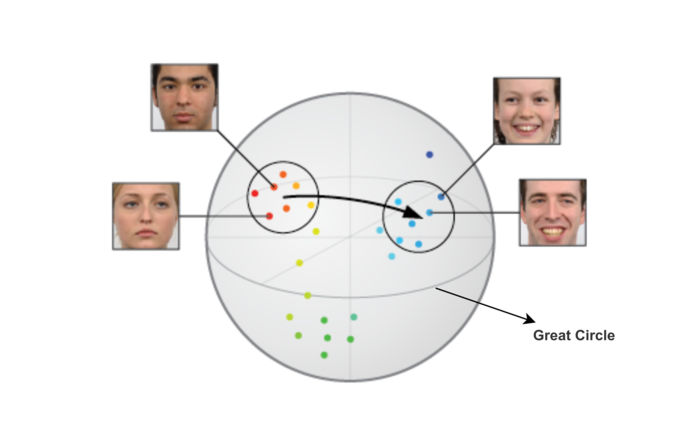
\includegraphics[width=\textwidth]{figures/background/sphericalZ.png}
    \caption{Illustration of the sampling from the great circle. Image source \cite{spherical_sampling}}
    \label{fig:great_circle}
\end{figure}

\paragraph{BatchNorm}
Training the \ac{gan} using separate batches of real and fake data without mixing them. And perform instance normalization when batch normalization is not possible.

\paragraph{Avoid Sparse Gradients}
Sparse gradients affect the training stability of the \ac{gan}. Hard functions like hard- \ac{relu}, Max Pooling that have sparse gradients should be avoided. Instead, Leaky-\ac{relu} work well for both the generator and the discriminator. And average pooling or convolution layers with stride are better for downsampling or upsampling.

As mentioned previously Tanh and Sigmoid activations are used for the output layers of the generator and the discriminator respectively. For all the remaining layers Leaky-\ac{relu} was tried and good results were observed. Experimenting with other combinations of activation functions, using Mish activation function \cite{mish} for the \ac{vae} and Leaky-\ac{relu} for the discriminator is found to give small but noticeable improvement to the performance.

Based on the choice of activation, Kaiming He initialization with Leaky-\ac{relu} non-linearity is used for all the layers.

\paragraph{Label Smooting}
The label smoothing technique mentioned in \cite{gan_hacks} is by replacing the binary labels for real and fake i.e 1, 0 with random numbers, between 0.7 and 1.2 and 0.0 to 0.3 respectively. However, there are different ways of doing smoothing. These include random/non-random, one-sided/two-sided, only for discriminator/both networks. Only the real labels are smoothed for both the discriminator and the generator in the experiments. 
% FIXME REDO mistake in implementation label smoothing only for D, not for G

\paragraph{Label Flipping}
The other way of making the labels noisy for the discriminator to prevent it from being too strong is by flipping labels during the discriminator training. Real labels are changed to fake and vice-versa occasionally to confuse the discriminator. 

This had some effect during the initial phase of the training but is not observed to directly affect the quantitative results and hence and kept inactive for simplicity.
% FIXME REDO experiment

\paragraph{GAN Model Choice} 
As training \acp{gan} is notoriously difficult, the most explored and studied variant DCGAN (Deep Convolutional \ac{gan}) is suggested to be used. The next best approach is to use hybrid models that use \ac{kld} or a combination of \ac{vae} and \ac{gan}. Since it is not desired to use convolutional layers in lifting networks, the proposed method is already following the best alternative.


\paragraph{Optimizer choice}
The best configuration of optimizers is Adam for the generator and SGD for the discriminator. However, this combination made the models diverge and has severely affected the training of the proposed method. Hence Adam is chosen for both the networks.

\paragraph{Noisy Inputs}
Adding noise to inputs and decaying over time helps the training. The 2D poses were added random noise in different scales but improvements were not noticeable in the basic experiments. 

\paragraph{Training Discriminator More}
To consistently get good feedback from the discriminator, it is ideal to keep always keep the discriminator at good performance. To achieve this, the discriminator is iterated $n$ times before every iteration of the \ac{vae}. However, $n$ is set to 1 as the benefit could not be seen in the initial observations.

\paragraph{Dropout}
Adding additional noise to the generator using dropout with $p=0.5$ during training and test time \cite{gan_dropout}. The discriminator uses dropout with $p=0.5$. But it is observed that adding dropout layers hurt \acp{vae} and $p=0.2$ was found to have a good trade-off. 

% \subsection{Model Summary}
% TODO wgan experiments 
% \section{Implementation}

% \lipsum[1] % FIXME
% \subsection{Monitoring}
% \lipsum[1] % FIXME

% \paragraph{use RL stability tricks} Not explored in this thesis. % TODO move to future

%TODO include flipping
